% Options for packages loaded elsewhere
\PassOptionsToPackage{unicode}{hyperref}
\PassOptionsToPackage{hyphens}{url}
%
\documentclass[
]{article}
\usepackage{amsmath,amssymb}
\usepackage{iftex}
\ifPDFTeX
  \usepackage[T1]{fontenc}
  \usepackage[utf8]{inputenc}
  \usepackage{textcomp} % provide euro and other symbols
\else % if luatex or xetex
  \usepackage{unicode-math} % this also loads fontspec
  \defaultfontfeatures{Scale=MatchLowercase}
  \defaultfontfeatures[\rmfamily]{Ligatures=TeX,Scale=1}
\fi
\usepackage{lmodern}
\ifPDFTeX\else
  % xetex/luatex font selection
\fi
% Use upquote if available, for straight quotes in verbatim environments
\IfFileExists{upquote.sty}{\usepackage{upquote}}{}
\IfFileExists{microtype.sty}{% use microtype if available
  \usepackage[]{microtype}
  \UseMicrotypeSet[protrusion]{basicmath} % disable protrusion for tt fonts
}{}
\makeatletter
\@ifundefined{KOMAClassName}{% if non-KOMA class
  \IfFileExists{parskip.sty}{%
    \usepackage{parskip}
  }{% else
    \setlength{\parindent}{0pt}
    \setlength{\parskip}{6pt plus 2pt minus 1pt}}
}{% if KOMA class
  \KOMAoptions{parskip=half}}
\makeatother
\usepackage{xcolor}
\usepackage[margin=1in]{geometry}
\usepackage{color}
\usepackage{fancyvrb}
\newcommand{\VerbBar}{|}
\newcommand{\VERB}{\Verb[commandchars=\\\{\}]}
\DefineVerbatimEnvironment{Highlighting}{Verbatim}{commandchars=\\\{\}}
% Add ',fontsize=\small' for more characters per line
\usepackage{framed}
\definecolor{shadecolor}{RGB}{248,248,248}
\newenvironment{Shaded}{\begin{snugshade}}{\end{snugshade}}
\newcommand{\AlertTok}[1]{\textcolor[rgb]{0.94,0.16,0.16}{#1}}
\newcommand{\AnnotationTok}[1]{\textcolor[rgb]{0.56,0.35,0.01}{\textbf{\textit{#1}}}}
\newcommand{\AttributeTok}[1]{\textcolor[rgb]{0.13,0.29,0.53}{#1}}
\newcommand{\BaseNTok}[1]{\textcolor[rgb]{0.00,0.00,0.81}{#1}}
\newcommand{\BuiltInTok}[1]{#1}
\newcommand{\CharTok}[1]{\textcolor[rgb]{0.31,0.60,0.02}{#1}}
\newcommand{\CommentTok}[1]{\textcolor[rgb]{0.56,0.35,0.01}{\textit{#1}}}
\newcommand{\CommentVarTok}[1]{\textcolor[rgb]{0.56,0.35,0.01}{\textbf{\textit{#1}}}}
\newcommand{\ConstantTok}[1]{\textcolor[rgb]{0.56,0.35,0.01}{#1}}
\newcommand{\ControlFlowTok}[1]{\textcolor[rgb]{0.13,0.29,0.53}{\textbf{#1}}}
\newcommand{\DataTypeTok}[1]{\textcolor[rgb]{0.13,0.29,0.53}{#1}}
\newcommand{\DecValTok}[1]{\textcolor[rgb]{0.00,0.00,0.81}{#1}}
\newcommand{\DocumentationTok}[1]{\textcolor[rgb]{0.56,0.35,0.01}{\textbf{\textit{#1}}}}
\newcommand{\ErrorTok}[1]{\textcolor[rgb]{0.64,0.00,0.00}{\textbf{#1}}}
\newcommand{\ExtensionTok}[1]{#1}
\newcommand{\FloatTok}[1]{\textcolor[rgb]{0.00,0.00,0.81}{#1}}
\newcommand{\FunctionTok}[1]{\textcolor[rgb]{0.13,0.29,0.53}{\textbf{#1}}}
\newcommand{\ImportTok}[1]{#1}
\newcommand{\InformationTok}[1]{\textcolor[rgb]{0.56,0.35,0.01}{\textbf{\textit{#1}}}}
\newcommand{\KeywordTok}[1]{\textcolor[rgb]{0.13,0.29,0.53}{\textbf{#1}}}
\newcommand{\NormalTok}[1]{#1}
\newcommand{\OperatorTok}[1]{\textcolor[rgb]{0.81,0.36,0.00}{\textbf{#1}}}
\newcommand{\OtherTok}[1]{\textcolor[rgb]{0.56,0.35,0.01}{#1}}
\newcommand{\PreprocessorTok}[1]{\textcolor[rgb]{0.56,0.35,0.01}{\textit{#1}}}
\newcommand{\RegionMarkerTok}[1]{#1}
\newcommand{\SpecialCharTok}[1]{\textcolor[rgb]{0.81,0.36,0.00}{\textbf{#1}}}
\newcommand{\SpecialStringTok}[1]{\textcolor[rgb]{0.31,0.60,0.02}{#1}}
\newcommand{\StringTok}[1]{\textcolor[rgb]{0.31,0.60,0.02}{#1}}
\newcommand{\VariableTok}[1]{\textcolor[rgb]{0.00,0.00,0.00}{#1}}
\newcommand{\VerbatimStringTok}[1]{\textcolor[rgb]{0.31,0.60,0.02}{#1}}
\newcommand{\WarningTok}[1]{\textcolor[rgb]{0.56,0.35,0.01}{\textbf{\textit{#1}}}}
\usepackage{graphicx}
\makeatletter
\newsavebox\pandoc@box
\newcommand*\pandocbounded[1]{% scales image to fit in text height/width
  \sbox\pandoc@box{#1}%
  \Gscale@div\@tempa{\textheight}{\dimexpr\ht\pandoc@box+\dp\pandoc@box\relax}%
  \Gscale@div\@tempb{\linewidth}{\wd\pandoc@box}%
  \ifdim\@tempb\p@<\@tempa\p@\let\@tempa\@tempb\fi% select the smaller of both
  \ifdim\@tempa\p@<\p@\scalebox{\@tempa}{\usebox\pandoc@box}%
  \else\usebox{\pandoc@box}%
  \fi%
}
% Set default figure placement to htbp
\def\fps@figure{htbp}
\makeatother
\setlength{\emergencystretch}{3em} % prevent overfull lines
\providecommand{\tightlist}{%
  \setlength{\itemsep}{0pt}\setlength{\parskip}{0pt}}
\setcounter{secnumdepth}{-\maxdimen} % remove section numbering
% definitions for citeproc citations
\NewDocumentCommand\citeproctext{}{}
\NewDocumentCommand\citeproc{mm}{%
  \begingroup\def\citeproctext{#2}\cite{#1}\endgroup}
\makeatletter
 % allow citations to break across lines
 \let\@cite@ofmt\@firstofone
 % avoid brackets around text for \cite:
 \def\@biblabel#1{}
 \def\@cite#1#2{{#1\if@tempswa , #2\fi}}
\makeatother
\newlength{\cslhangindent}
\setlength{\cslhangindent}{1.5em}
\newlength{\csllabelwidth}
\setlength{\csllabelwidth}{3em}
\newenvironment{CSLReferences}[2] % #1 hanging-indent, #2 entry-spacing
 {\begin{list}{}{%
  \setlength{\itemindent}{0pt}
  \setlength{\leftmargin}{0pt}
  \setlength{\parsep}{0pt}
  % turn on hanging indent if param 1 is 1
  \ifodd #1
   \setlength{\leftmargin}{\cslhangindent}
   \setlength{\itemindent}{-1\cslhangindent}
  \fi
  % set entry spacing
  \setlength{\itemsep}{#2\baselineskip}}}
 {\end{list}}
\usepackage{calc}
\newcommand{\CSLBlock}[1]{\hfill\break\parbox[t]{\linewidth}{\strut\ignorespaces#1\strut}}
\newcommand{\CSLLeftMargin}[1]{\parbox[t]{\csllabelwidth}{\strut#1\strut}}
\newcommand{\CSLRightInline}[1]{\parbox[t]{\linewidth - \csllabelwidth}{\strut#1\strut}}
\newcommand{\CSLIndent}[1]{\hspace{\cslhangindent}#1}
\usepackage{bookmark}
\IfFileExists{xurl.sty}{\usepackage{xurl}}{} % add URL line breaks if available
\urlstyle{same}
\hypersetup{
  pdftitle={Statistical Analysis of Alberta Wildfires from (2006 - 2024)},
  hidelinks,
  pdfcreator={LaTeX via pandoc}}

\title{Statistical Analysis of Alberta Wildfires from (2006 - 2024)}
\author{Group4: Johanna Enright - 30303537, Uyoyoumena Orona - 30295200,
Agambir Bandesha - 30302510, Ran Bi - 30301306}
\date{Date: 2025-10-04}

\begin{document}
\maketitle

\section{Abstract}\label{abstract}

\begin{itemize}
\tightlist
\item
  maybe we want an abstract (which we will write at the end)?
\end{itemize}

\section{Introduction}\label{introduction}

\indent In Canada and across the world, we have seen an increase in
forest area burned due to forest fires, with 2023 being an a record
breaking year in forest damage for Canada (MacCarthy et al., 2025).
Climate change is the main culprit, with changing weather patterns
bringing heatwaves and drought which makes forests more easily ignitable
than in the past (MacCarthy et al., 2025). Wildfires can be devastating
to the forest ecosystem, but they also can have large ramifications on
the economy and human health (Sadof \& Anderson, 2023). When forests are
burned, carbon dioxide is released into the air, further exacerbating
our climate crisis and creating a positive feedback loop for future
disastrous wildfires (Sadof \& Anderson, 2023). Scientists have made
significant efforts to understand forest fire dynamics allowing for
improved forest fire mitigation and combative tactics \emph{cite?}.
However, it is of great importance to continue to research and
understand how the forest fire landscape in Canada is changing so we can
be better prepared to mitigate the environmental, economic, and social
damages they will cause.

\section{1. Purpose}\label{purpose}

\subsection{Domain:}\label{domain}

\indent Our project looks at forest fire data in Alberta between 2006
and 2024. The data set gives information on total area burned, fire
spread rate, causes of fires, as well as fire types, and time stamps and
location coordinates {Forestry \& Parks (2025)}. We are narrowing our
focus down to specifically focus on how weather factors, like wind
speed, contribute to fire spread rate as well as how the cause of fires
(specifically lightning) may be changing over time due to climate
change.

\subsection{Investigation Goal:}\label{investigation-goal}

\indent **Question 1:** Research has indicated that the frequency of
lightning caused forest fires is increasing due to climate change
{Beverly (2024)}. We want to see if the Alberta forest fire data
corroborates this claim. We will compare the difference between the
estimated proportion of lightning caused wildfires from 2024 to the
estimated proportion of lightning caused wildfires from 2006 to see if
the former is significantly larger than the latter.

\indent **Question 2:** There are a variety of environmental factors
which affect how quickly a fire spreads, ultimately contributing to the
overall impact and environmental burden that a forest fire has on its
surrounding area. We are investigating how one key weather variable,
wind speed, affects the fire spread rate.

\subsection{Practical Implications: \#We can expand on this
section}\label{practical-implications-we-can-expand-on-this-section}

\indent **Question 1**: By examining how the proportion of
lightning-caused wildfires has changed over time, we can assess one way
in which climate change is reshaping wildfire patterns. In Canada,
lightning already causes almost half of all wildfires and accounts for
about 90\% of burned forest area {Coogan et al. (2025)}. Climate change
is increasing both lightning frequency and the amount of dry, flammable
debris in forests {Public Health Agency of Canada (2024)}, suggesting
more lightning-driven fires in the future. Examining these trends helps
estimate climate impacts, inform on fossil fuel emission-reduction
policies, and guide forest management practices such as prescribed
burning {Parks Canada (2025)}.

\indent **Question 2**: We are investigating how wind speed affects fire
spread. In reality, wildfire models also include factors like humidity,
temperature, topography, and fuel type (Natural Resources Canada, 2025).
Understanding how wind accelerates the rate of fire spread helps predict
fire risk to communities and habitats, guide evacuation needs, and
assess environmental and economic impacts. High winds can also reduce
the effectiveness of aerial fire suppression, making wind speed a key
factor to understand in wildfire management {Shmuel \& Heifetz (2023)}.

\subsection{Population(s) of Interest:}\label{populations-of-interest}

\indent Our forest fire data set looks at wildfires in Alberta between
2006 and 2024. Specifically this data includes wildfires only occurring
within the FPA (forest protection area), either provincial or federally
owned/managed lands. For question 1, we will investigate forest fires in
2006 and 2024, with 1954 and 1230 wildfire entries, respectively. We
will be comparing forest fires caused by lightning to those caused by
all non-natural human activity. For question 2, we will study all forest
fire entries that contain information for fire spread rate and wind
speed. This accounts for around 89\% \(\frac{23657}{26551}\) of data
entries.

\subsection{Variables of Interest:}\label{variables-of-interest}

\indent **Question 1:** The variables we will analyze are fires within
the ``GENERAL\_CAUSE'' column of the data set which are ``Lightning'' (1
Success). All other fires within the ``GENERAL\_CAUSE'' column which are
not ``Lightning'' will be considered a 0 (Failure). We will analyze this
variable for fires in the ``YEAR'' 2024 and compare it to fires from the
``YEAR'' 2006. \indent **Question 2**: For the linear regression, our
independent (x) variable will be the numerical variable ``WIND\_SPEED''
(in km/h) and our dependant (y) variable will be the numerical variable
``FIRE\_SPREAD\_RATE'' (in m/min).

\subsection{Data Collection Method:}\label{data-collection-method}

\indent **Quesetion 1**. The ``GENERAL\_CAUSE'' of wildfires is
investigated by Alberta wildfire officials. Wildfires under
investigation where the cause was not determined were labelled
``Undetermined''. \indent *Question 2*. ``FIRE\_SPREAD\_RATE'' and
``WIND\_SPEED'' were recorded at the time of initial fire assessment.
The exact assessors are Alberta Wildfire personnel and are indicated in
the ``ASSESSMENT\_RESOURCE'' column of the data set who assessed the
fire at the recorded ``ASSESSMENT\_DATETIME''. Assessors include ``air
attack officer'', ``initial action forces'', ``wildfire assessor'', or
``other''. More details on these assessment positions can be found in
the Historical Wildfire Data Dictionary (Forestry and Parks, 2025).

\section{2. Data}\label{data}

\subsection{Source of Data:}\label{source-of-data}

\indent This data comes from the Government of Alberta official website,
published by Forestry and Parks. The full data set name is Historical
wildfire data: 2006 to 2024.

\subsection{Data Characteristics:}\label{data-characteristics}

\textbf{{[}Describe the nature of the data (e.g., categorical,
continuous, time-series, text/unstructured) and the primary variables
you will be using{]}} \textbf{New section}

\subsection{Permission/Accessibility:}\label{permissionaccessibility}

\indent This data set contains information licensed under the Open
Government Licence - Alberta. This worldwide, royalty-free, perpetual,
non-exclusive license allows us to copy, modify, publish, translate,
adapt, distribute or otherwise use the information in any medium, mode
or format for any lawful purpose {Government of Alberta (n.d.)}.

\subsection{Time Frame of Data Collection
:}\label{time-frame-of-data-collection}

\indent Data was collected from 2006-01-01 to 2024-12-31. The resource
was created on 2020-01-09 and was last modified on 2025-01-31. Updates
to this data set are irregular in frequency.

\section{3. Topic(s) to Investigate}\label{topics-to-investigate}

\indent **Question 1**: We want to see if the proportion of lightning
caused wildfires from 2024 is significantly greater than the proportion
of lightning caused wildfires from 2006. We hypothesize that 2024 will
have a significantly higher proportion than wildfires from 2006 due to
climate change which has resulted in a higher frequency of lightning
strikes, and drier forest conditions beneficial for fire ignition upon a
lightning strike. We will assess if
\(p_{lightning, 2024} > p_{lightning, 2006}\) as outlined by our
hypotheses below. \[
H_{0} :         p_{lightning, 2024} \leq p_{lightning, 2006} \\
H_{A}:  p_{lightning, 2024}  > p_{lightning, 2006}
\]

\indent **Question 2**: Wildfires are a persistent threat globally, with
significant social, ecological, and economic impacts. Their spread and
intensity result from complex interactions among fuels, topography,
weather, and especially wind speed. This project will investigate the
statistical relationship between wind speed and fire spread rate using
historical wildfire data from 2006--2024. The primary research question
asks: To what extent does wind speed predict the rate of wildfire
spread? Understanding this relationship holds practical implications for
fire behavior prediction, risk management, and the development of early
warning systems for communities in wildfire-prone regions.

The population of interest includes all historical wildfires recorded
within the provided dataset, with key variables being fire spread rate
and wind speed. Both variables have been observed and recorded during
wildfire events, with data carefully logged.

Wildfires are a recurring natural hazard in Alberta, Canada, where vast
boreal forests, grasslands, and mixed-fuel landscapes are exposed to
seasonal fire risk. Between 2006 and 2024, over 26,000 fire events were
recorded in the Historical Wildfire Data data set (Forestry \& Parks,
2025). This data set provides a unique opportunity to study the
environmental drivers of fire behaviour in a consistent, long-term
record. In Alberta, major fire events such as the 2016 Fort McMurray
wildfire highlighted how fast-spreading fires can destroy thousands of
structures, displace tens of thousands of people, and cost billions in
recovery. Anticipating spread rate is therefore a central concern in
wildfire management, where even small gains in prediction can inform
life-saving interventions. Research shows that wildfire spread is
influenced by a combination of fuels, weather, and topography (Canada,
2025). Among these, wind speed is consistently identified as one of the
strongest drivers. Higher winds tilt flames forward, enhance radiant and
convective heating of unburned fuels, and carry embers downwind, which
accelerates the head fire and can ignite spot fires well ahead of the
main front (Rothermel, 1972). Wind speed is also operationally relevant
because it constrains firefighting tactics. Strong winds reduce the
accuracy and effectiveness of aerial suppression, causing water and
retardant drops to drift away from the target (Fogarty \& Slijepcevic,
1997; Plucinski et al., 2025). They also increase risks to ground crews
and limit the safe use of heavy equipment. Thus, understanding how
spread responds to wind speed not only improves predictive science but
also shapes suppression planning and resource allocation. In this
project, we therefore hypothesize that wind speed will be a largely
contributing factor to fire spread rate in Alberta. To test this, we
will fit a simple linear regression model of the form:
FIRE\_SPREAD\_RATE \textasciitilde{} WIND\_SPEED

\begin{center}
$H_{0}:$ There is no correlation between wind speed and fire spread rate. \\
$H_{A}:$ The alternative hypothesis is a correlation between wind speed and fire spread rate.
\end{center}

\section{4. Statistical Methods}\label{statistical-methods}

\subsection{Planned Methods:}\label{planned-methods}

\indent **Question 1** : We will use a classical right sided Z test for
proportions to determine if
\(p_{lightning, 2024} > p_{lightning, 2006}\) as determined by the
formula: \[
Z_{obs}=\frac{(\widehat{p}_{1}-\widehat{p}_{2})-(p_{1}-p_{2})}{(p(1-p)(\frac{1}{n_{1}}+\frac{1}{n_{1}})}   \\
\text{where }   p=\frac{x_{1}+x_{2}}{n_{1} + n_{2}}  \quad
\text{  and }\quad p_{1}-p_{2} = 0  \text{ under the null hypothesis.}
\] We will reject the null hypothesis if \(p < 0.05\). We have confirmed
that the conditions to use this method are met. Our variables
\(p_{lightning, 2024} > p_{lightning, 2006}\) are from independent
samples. Our n values are sufficiently large with
\(n_{2024} = 1230 \text{ and } n_{2006} = 1954\) to use parametric tests
relying on the central limit theorem. To confirm our methods, we will
also use the conventional \(\frac{+1}{+2}\) Agresti-coull confidence
interval for the difference between proportions. \[
(\tilde{p}_{1}- \tilde{p}_{2}) \space\pm\space
z_{1-2/\alpha}
\sqrt{\frac{\tilde{p}_{1}(1-\tilde{p}_{1})}{n_{1}+2}+\frac{\tilde{p}_{2}(1-\tilde{p}_{2})}{n_{2} + 2}} \\
\text{where}\quad   \tilde{p}_{1} = \frac{X_{1}+1}{n_1+2}  \quad\text{and}\quad    \tilde{p}_{2} =\frac{ X_{2}+1}{n_2+2}
\] We will compute this confidence interval for
\(p_{lightning, 2024} - p_{lightning, 2006}\) and if both bounds of the
confidence interval are above 0, this will confirm that we should reject
the null hypothesis and conclude that
\(p_{lightning, 2024}  > p_{lightning, 2006}\). If the bounds encompass
0, we will conclude that there is no significant difference between
\(p_{lightning, 2024}  \text{ and } p_{lightning, 2006}\).

\indent **Question 2** : Our aim is to estimate the strength and nature
of the relationship between wind speed and fire spread rate using a
simple linear regression. \[
Y_{i} = \beta_{0} + \beta_{1}x_{i} + \epsilon_{i}
\]

\begin{flushleft}
where: \\
* $i =$ fire spread rate for the $i_{th}$ observation. \\
* $x_{i} =$ wind speed for the $i_{th}$ observation. \\
* $\beta_{0}$ = intercept (the estimated fire spread rate when wind speed is 0). \\
* $\beta_{1}$ = slope (the expected change in fire spread rate for a one-unit increase in wind speed). \\
* $\epsilon_{i}$ = random error term accounting for variation not explained by wind speed.
\end{flushleft}

We will estimate \(\beta_{0}\) and \(\beta_{1}\) using least squares
regression, which minimizes the sum of squared differences between
observed fire spread rates and predicted values.

\begin{flushleft}
The null hypothesis is $H_{0}:  \beta_{1} = 0$
The alternative hypothesis is $H_{A}: \beta_{1} \ne 0$
\end{flushleft}

We will then assess the strength of the relationship using: - The
estimated slope \(\beta_{1}\) - The coefficient of determination (R2),
which measures how much of the variation in fire spread rate is
explained by wind speed. In the end, we will also utilize a residual
plot to assess our regression.

\section{5. Results}\label{results}

We will investigate our initial question to see if the proportion of
lightning-caused forest fires is significantly greater in 2024 than it
is in 2006.

The initial sample proportions for each year are 0.38 and 0.45 for the
year 2006 and 2024 respectively (Figure @ref(fig:piechart)).

\begin{figure}
\centering
\pandocbounded{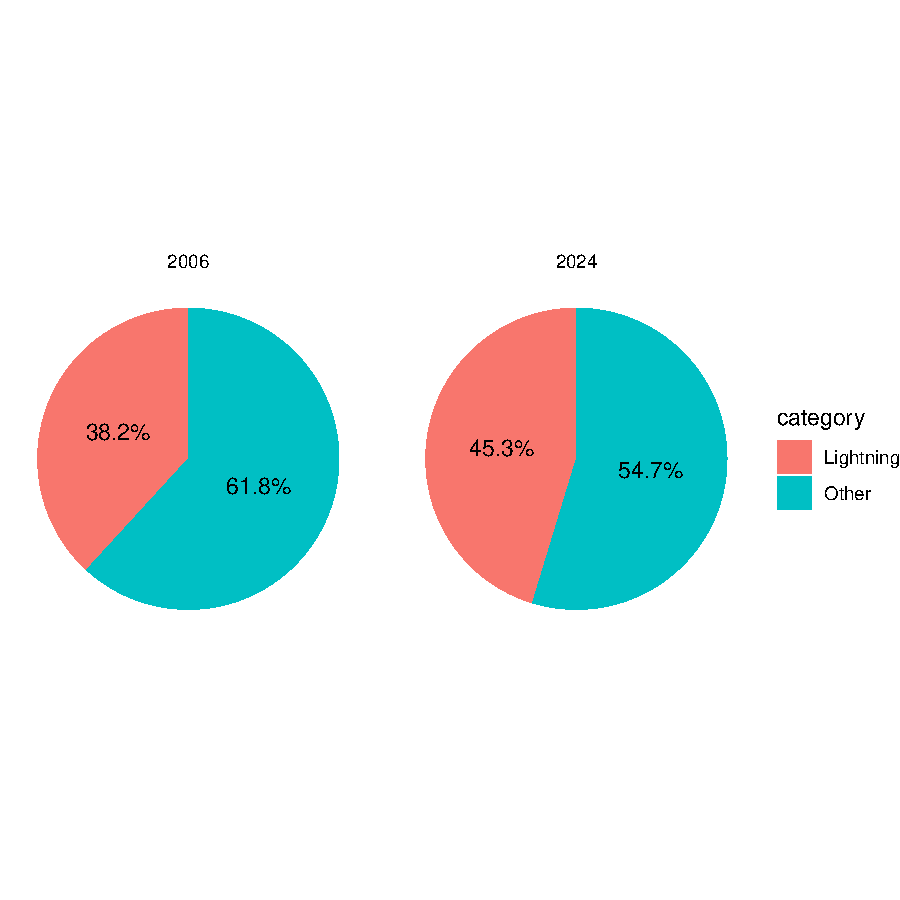
\includegraphics[keepaspectratio]{602_Report_files/figure-latex/piechart-1.pdf}}
\caption{Proportion of Lightning-Caused Fires in 2006 and 2024}
\end{figure}

Next we will confirm that our data follows the assumptions necessary to
use a parametric test. (i.e.~that n is sufficiently large under the
central limit theorem).

Confirmed here, all values of n are sufficiently large to use the
central limit theorem tests.

Testing hypothesis \(H_{0}: p_{2024} \leq p_{2006}\) and
\(H_{A}: p_{2024} > p_{2006}\)

\begin{Shaded}
\begin{Highlighting}[]
\DocumentationTok{\#\#\#\#\#\#\#\#\#\#\#\#\#\#\#\#\#\#\#\#\#\#\#\#\#\#\#\#\#  CALCULATING Z{-}observed \#\#\#\#\#\#\#\#\#\#\#\#\#\#\#\#\#\#\#\#\#\#\#\#\#\#\#\#\#\#\#\#\#\#\#\#}
\NormalTok{phat }\OtherTok{\textless{}{-}}\NormalTok{ (x\_2006 }\SpecialCharTok{+}\NormalTok{ x\_2024)}\SpecialCharTok{/}\NormalTok{(n\_2006 }\SpecialCharTok{+}\NormalTok{ n\_2024)}
\NormalTok{p1\_min\_p2 }\OtherTok{\textless{}{-}} \DecValTok{0}   \CommentTok{\#under the assumption of the null hypothesis}
\NormalTok{Zobs }\OtherTok{\textless{}{-}}\NormalTok{ ((p\_lightning\_2024 }\SpecialCharTok{{-}}\NormalTok{ p\_lightning\_2006) }\SpecialCharTok{{-}}\NormalTok{ p1\_min\_p2)}\SpecialCharTok{/}\FunctionTok{sqrt}\NormalTok{(phat}\SpecialCharTok{*}\NormalTok{(}\DecValTok{1}\SpecialCharTok{{-}}\NormalTok{phat)}\SpecialCharTok{*}\NormalTok{(}\DecValTok{1}\SpecialCharTok{/}\NormalTok{n\_2024 }\SpecialCharTok{+} \DecValTok{1}\SpecialCharTok{/}\NormalTok{n\_2006))}
\NormalTok{pvalue }\OtherTok{\textless{}{-}} \FunctionTok{round}\NormalTok{(}\DecValTok{1} \SpecialCharTok{{-}} \FunctionTok{pnorm}\NormalTok{(Zobs),}\DecValTok{5}\NormalTok{)}
\FunctionTok{print}\NormalTok{(}\FunctionTok{paste}\NormalTok{(}\StringTok{"The test statistic is:"}\NormalTok{, }\FunctionTok{round}\NormalTok{(Zobs,}\DecValTok{4}\NormalTok{), }\StringTok{"The p{-}value is:"}\NormalTok{, pvalue))}
\end{Highlighting}
\end{Shaded}

\begin{verbatim}
## [1] "The test statistic is: 3.9418 The p-value is: 4e-05"
\end{verbatim}

Therefore, because our p-value is less than our alpha of 0.05, we can
conclude that the proportion of lightning caused wildfires in 2024 is
significantly greater than the proportion from 2006.

\pandocbounded{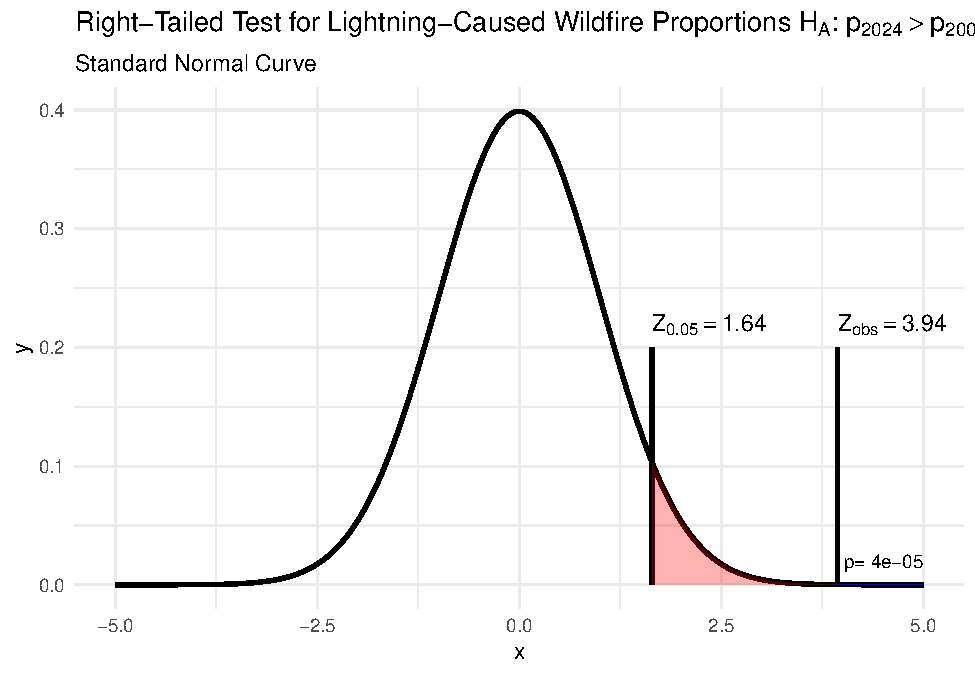
\includegraphics[keepaspectratio]{602_Report_files/figure-latex/unnamed-chunk-5-1.pdf}}

Next, we will confirm our findings with a 95\% Agresti-Coull Confidence
interval for the difference in proportions, \(p_{2024}-p_{2006}\).

\begin{Shaded}
\begin{Highlighting}[]
\DocumentationTok{\#\#\#\#\#\#\#\#\#\#\#\#\#\#\#\#\#\# USING THE AGRESTI{-}COULL (+1/+2 METHOD) 95\% CI \#\#\#\#\#\#\#\#\#\#\#\#\#\#\#\#\#\#\#\#\#\#\#\#\#\#\#\#\#\#\#\#}
\NormalTok{p\_tilde\_2024 }\OtherTok{\textless{}{-}}\NormalTok{ (x\_2024 }\SpecialCharTok{+} \DecValTok{1}\NormalTok{)}\SpecialCharTok{/}\NormalTok{(n\_2024 }\SpecialCharTok{+} \DecValTok{2}\NormalTok{)}
\NormalTok{p\_tilde\_2006 }\OtherTok{\textless{}{-}}\NormalTok{ (x\_2006 }\SpecialCharTok{+} \DecValTok{1}\NormalTok{)}\SpecialCharTok{/}\NormalTok{(n\_2006 }\SpecialCharTok{+} \DecValTok{2}\NormalTok{)}

\NormalTok{ptilde\_diff }\OtherTok{\textless{}{-}}\NormalTok{ p\_tilde\_2024 }\SpecialCharTok{{-}}\NormalTok{ p\_tilde\_2006}
\NormalTok{z }\OtherTok{\textless{}{-}} \FunctionTok{qnorm}\NormalTok{(}\DecValTok{1} \SpecialCharTok{{-}} \FloatTok{0.05}\SpecialCharTok{/}\DecValTok{2}\NormalTok{)}
\NormalTok{SE }\OtherTok{\textless{}{-}} \FunctionTok{sqrt}\NormalTok{(((p\_tilde\_2024)}\SpecialCharTok{*}\NormalTok{(}\DecValTok{1}\SpecialCharTok{{-}}\NormalTok{p\_tilde\_2024)}\SpecialCharTok{/}\NormalTok{(n\_2024 }\SpecialCharTok{+} \DecValTok{2}\NormalTok{)) }\SpecialCharTok{+}
\NormalTok{            ((p\_tilde\_2006)}\SpecialCharTok{*}\NormalTok{(}\DecValTok{1}\SpecialCharTok{{-}}\NormalTok{p\_tilde\_2006)}\SpecialCharTok{/}\NormalTok{(n\_2006 }\SpecialCharTok{+} \DecValTok{2}\NormalTok{))}
\NormalTok{                )}

\NormalTok{lb }\OtherTok{\textless{}{-}}\NormalTok{ ptilde\_diff }\SpecialCharTok{{-}}\NormalTok{ z }\SpecialCharTok{*}\NormalTok{ SE}
\NormalTok{ub }\OtherTok{\textless{}{-}}\NormalTok{ ptilde\_diff }\SpecialCharTok{+}\NormalTok{ z }\SpecialCharTok{*}\NormalTok{ SE}
\FunctionTok{paste}\NormalTok{(}\FunctionTok{round}\NormalTok{(lb, }\DecValTok{4}\NormalTok{), }\StringTok{"{-}"}\NormalTok{, }\FunctionTok{round}\NormalTok{(ub, }\DecValTok{4}\NormalTok{))}
\end{Highlighting}
\end{Shaded}

\begin{verbatim}
## [1] "0.0353 - 0.1057"
\end{verbatim}

\begin{Shaded}
\begin{Highlighting}[]
\CommentTok{\# CONCLUSION : 2024 HAS A SIGNIFICANTLY HIGHER PROPORITON OF LIGHTNING{-}CAUSED WILDFIRES THAT 2006}
\end{Highlighting}
\end{Shaded}

Our 95\% confidence interval for \(p_{2024}-p_{2006}\) lies between
0.0353 - 0.1057. Both lower and upper bounds of our confidence interval
are greater than 0, so this supports the above conclusion that the
proportion of lightning caused wildfires from 2024 is significantly
greater than that of 2006.

Here is a visualization for our 95\% confidence interval.

\pandocbounded{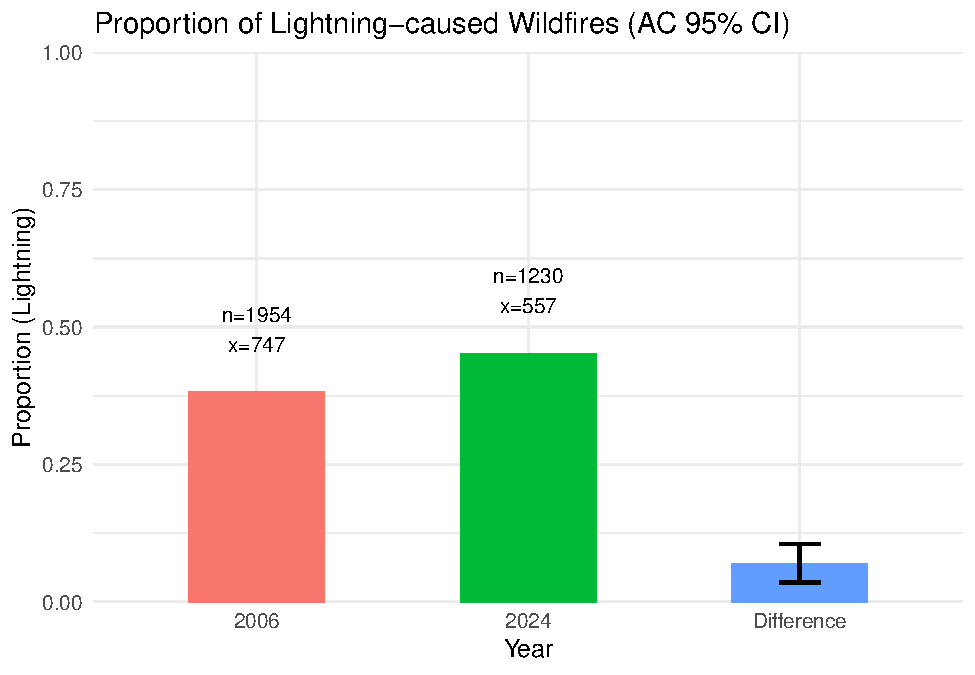
\includegraphics[keepaspectratio]{602_Report_files/figure-latex/unnamed-chunk-7-1.pdf}}

\subsection{Question 2}\label{question-2}

\begin{Shaded}
\begin{Highlighting}[]
\CommentTok{\# Create a clean dataset with only complete cases}
\NormalTok{wildfire\_clean }\OtherTok{=}\NormalTok{ df }\SpecialCharTok{\%\textgreater{}\%}  \FunctionTok{filter}\NormalTok{(}\SpecialCharTok{!}\FunctionTok{is.na}\NormalTok{(WIND\_SPEED) }\SpecialCharTok{\&} \SpecialCharTok{!}\FunctionTok{is.na}\NormalTok{(FIRE\_SPREAD\_RATE))}
\CommentTok{\# Use the clean dataset}
\NormalTok{lm\_model }\OtherTok{=} \FunctionTok{lm}\NormalTok{(FIRE\_SPREAD\_RATE }\SpecialCharTok{\textasciitilde{}}\NormalTok{ WIND\_SPEED, }\AttributeTok{data =}\NormalTok{ wildfire\_clean)}
\FunctionTok{summary}\NormalTok{(lm\_model)}
\end{Highlighting}
\end{Shaded}

\begin{verbatim}
## 
## Call:
## lm(formula = FIRE_SPREAD_RATE ~ WIND_SPEED, data = wildfire_clean)
## 
## Residuals:
##    Min     1Q Median     3Q    Max 
## -4.351 -0.871 -0.601  0.044 99.256 
## 
## Coefficients:
##             Estimate Std. Error t value Pr(>|t|)    
## (Intercept) 0.531468   0.024340   21.84   <2e-16 ***
## WIND_SPEED  0.042441   0.001993   21.30   <2e-16 ***
## ---
## Signif. codes:  0 '***' 0.001 '**' 0.01 '*' 0.05 '.' 0.1 ' ' 1
## 
## Residual standard error: 2.577 on 23655 degrees of freedom
## Multiple R-squared:  0.01882,    Adjusted R-squared:  0.01878 
## F-statistic: 453.7 on 1 and 23655 DF,  p-value: < 2.2e-16
\end{verbatim}

\begin{verbatim}
## `geom_smooth()` using formula = 'y ~ x'
\end{verbatim}

\pandocbounded{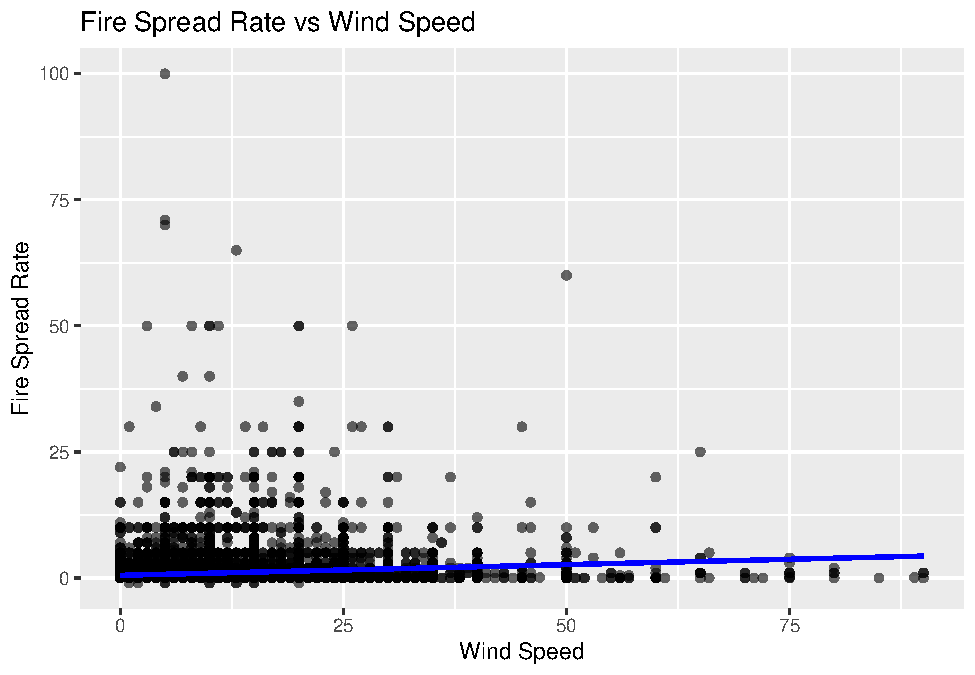
\includegraphics[keepaspectratio]{602_Report_files/figure-latex/unnamed-chunk-9-1.pdf}}
\pandocbounded{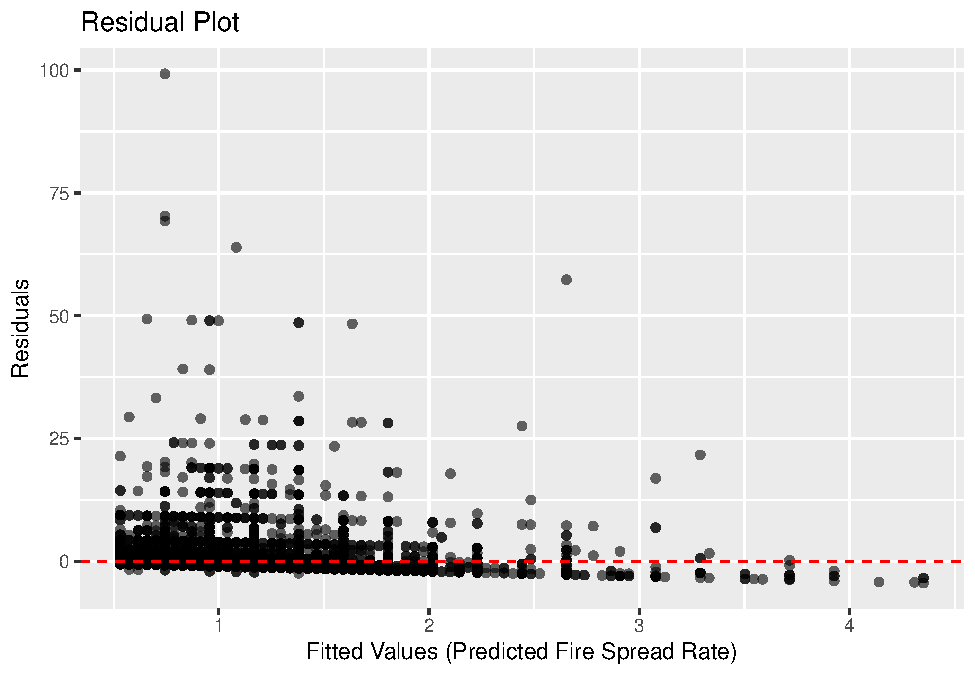
\includegraphics[keepaspectratio]{602_Report_files/figure-latex/unnamed-chunk-9-2.pdf}}

\begin{verbatim}
## Total observations in dataset: 26551
\end{verbatim}

\begin{verbatim}
## Complete cases used in analysis: 23657
\end{verbatim}

\begin{verbatim}
## Observations removed due to missing data: 2894
\end{verbatim}

\pandocbounded{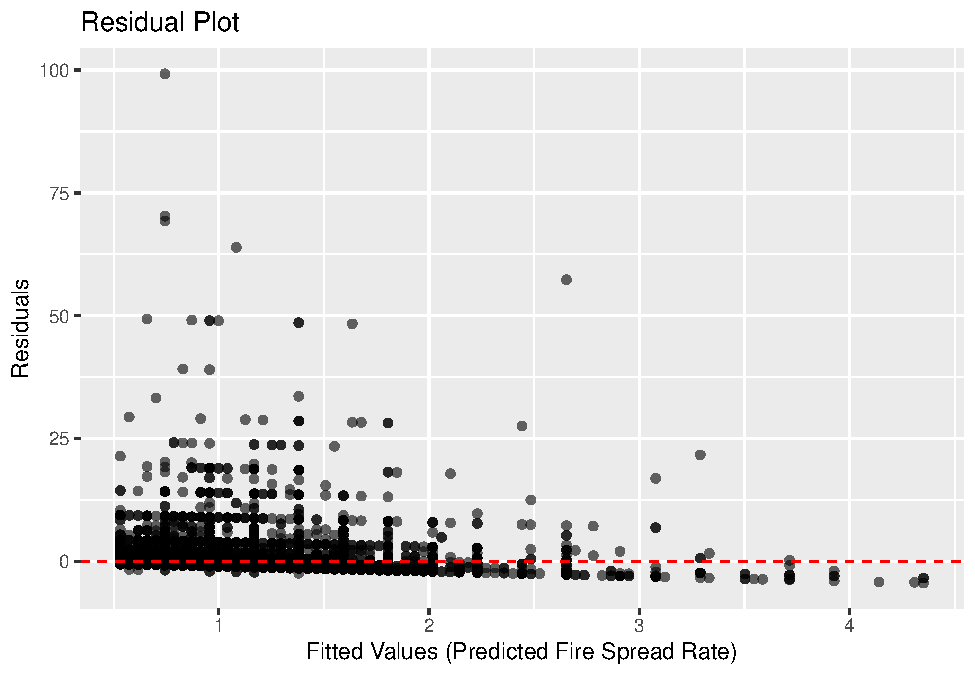
\includegraphics[keepaspectratio]{602_Report_files/figure-latex/unnamed-chunk-10-1.pdf}}

\begin{verbatim}
## Total observations in dataset: 26551
\end{verbatim}

\begin{verbatim}
## Complete cases used in analysis: 23657
\end{verbatim}

\begin{verbatim}
## Observations removed due to missing data: 2894
\end{verbatim}

\section{Conclusion And Future Work}\label{conclusion-and-future-work}

6.1 Interpretation of Results {[}Discuss what the results imply in the
context of the research questions and domain.{]} 6.2 Limitations
{[}Highlight any limitations of the data or methodology that may impact
conclusions.{]} 6.3 Recommendations and Future Directions {[}Suggest
potential extensions of the study, alternative methods, or further
investigations that could build on your findings.{]}

\section{References}\label{references}

\#Appendix

Here is some additional code that was not shown in the report

\begin{Shaded}
\begin{Highlighting}[]
\CommentTok{\# Visualization for difference in proportions}
\NormalTok{plot\_df }\OtherTok{\textless{}{-}} \FunctionTok{tibble}\NormalTok{(}
  \AttributeTok{YEAR  =} \FunctionTok{factor}\NormalTok{(}\FunctionTok{c}\NormalTok{(}\DecValTok{2006}\NormalTok{, }\DecValTok{2024}\NormalTok{, }\StringTok{"Difference"}\NormalTok{)),}
  \AttributeTok{prop  =} \FunctionTok{c}\NormalTok{(p\_lightning\_2006, p\_lightning\_2024, p\_lightning\_2024}\SpecialCharTok{{-}}\NormalTok{p\_lightning\_2006),}
  \AttributeTok{lower =} \FunctionTok{c}\NormalTok{(}\ConstantTok{NA}\NormalTok{, }\ConstantTok{NA}\NormalTok{, lb),}
  \AttributeTok{upper =} \FunctionTok{c}\NormalTok{(}\ConstantTok{NA}\NormalTok{, }\ConstantTok{NA}\NormalTok{, ub),}
  \AttributeTok{n     =} \FunctionTok{c}\NormalTok{(n\_2006, n\_2024, }\ConstantTok{NA}\NormalTok{),}
  \AttributeTok{x     =} \FunctionTok{c}\NormalTok{(x\_2006, x\_2024, }\ConstantTok{NA}\NormalTok{)}
\NormalTok{)}

\FunctionTok{ggplot}\NormalTok{(plot\_df, }\FunctionTok{aes}\NormalTok{(}\AttributeTok{x =}\NormalTok{ YEAR, }\AttributeTok{y =}\NormalTok{ prop, }\AttributeTok{fill =}\NormalTok{ YEAR)) }\SpecialCharTok{+}
  \FunctionTok{geom\_col}\NormalTok{(}\AttributeTok{width =} \FloatTok{0.5}\NormalTok{, }\AttributeTok{show.legend =} \ConstantTok{FALSE}\NormalTok{) }\SpecialCharTok{+}
  \FunctionTok{geom\_errorbar}\NormalTok{(}\FunctionTok{aes}\NormalTok{(}\AttributeTok{ymin =}\NormalTok{ lower, }\AttributeTok{ymax =}\NormalTok{ upper), }\AttributeTok{width =} \FloatTok{0.15}\NormalTok{, }\AttributeTok{linewidth =} \FloatTok{0.8}\NormalTok{) }\SpecialCharTok{+}
  \FunctionTok{geom\_text}\NormalTok{(}\FunctionTok{aes}\NormalTok{(}\AttributeTok{label =} \FunctionTok{ifelse}\NormalTok{(YEAR }\SpecialCharTok{\%in\%} \FunctionTok{c}\NormalTok{(}\DecValTok{2006}\NormalTok{, }\DecValTok{2024}\NormalTok{), }\FunctionTok{paste0}\NormalTok{(}\StringTok{"n="}\NormalTok{, n, }\StringTok{"}\SpecialCharTok{\textbackslash{}n}\StringTok{x="}\NormalTok{, x), }\ConstantTok{NA}\NormalTok{)),}
            \AttributeTok{vjust =} \SpecialCharTok{{-}}\FloatTok{0.9}\NormalTok{, }\AttributeTok{size =} \FloatTok{3.5}\NormalTok{) }\SpecialCharTok{+}
  \FunctionTok{scale\_y\_continuous}\NormalTok{(}\AttributeTok{limits =} \FunctionTok{c}\NormalTok{(}\DecValTok{0}\NormalTok{, }\DecValTok{1}\NormalTok{), }\AttributeTok{expand =} \FunctionTok{c}\NormalTok{(}\DecValTok{0}\NormalTok{, }\DecValTok{0}\NormalTok{)) }\SpecialCharTok{+}
  \FunctionTok{labs}\NormalTok{(}
    \AttributeTok{title =} \StringTok{"Proportion of Lightning{-}caused Wildfires (AC 95\% CI)"}\NormalTok{,}
    \AttributeTok{x =} \StringTok{"Year"}\NormalTok{,}
    \AttributeTok{y =} \StringTok{"Proportion (Lightning)"}
\NormalTok{  ) }\SpecialCharTok{+}
  \FunctionTok{theme\_minimal}\NormalTok{(}\AttributeTok{base\_size =} \DecValTok{12}\NormalTok{)}
\end{Highlighting}
\end{Shaded}

\begin{Shaded}
\begin{Highlighting}[]
\CommentTok{\#Script for right{-}tailed test visualization}
\NormalTok{x }\OtherTok{\textless{}{-}} \FunctionTok{seq}\NormalTok{(}\SpecialCharTok{{-}}\DecValTok{5}\NormalTok{, }\DecValTok{5}\NormalTok{,}\FloatTok{0.001}\NormalTok{)}
\NormalTok{df\_norm }\OtherTok{\textless{}{-}} \FunctionTok{tibble}\NormalTok{(}\AttributeTok{x =}\NormalTok{ x, }\AttributeTok{y =} \FunctionTok{dnorm}\NormalTok{(x, }\AttributeTok{mean =} \DecValTok{0}\NormalTok{, }\AttributeTok{sd =} \DecValTok{1}\NormalTok{))}

\CommentTok{\#labels for lines}
\NormalTok{labels\_df }\OtherTok{\textless{}{-}} \FunctionTok{tibble}\NormalTok{(}\AttributeTok{x =} \FunctionTok{c}\NormalTok{(}\FunctionTok{qnorm}\NormalTok{(}\FloatTok{0.95}\NormalTok{), Zobs), }\AttributeTok{y =} \FloatTok{0.21}\NormalTok{,}
                 \AttributeTok{label =} \FunctionTok{c}\NormalTok{(}\FunctionTok{bquote}\NormalTok{(Z[}\FloatTok{0.05}\NormalTok{] }\SpecialCharTok{==}\NormalTok{ .(}\FunctionTok{round}\NormalTok{(}\FunctionTok{qnorm}\NormalTok{(}\FloatTok{0.95}\NormalTok{),}\DecValTok{2}\NormalTok{))), }\FunctionTok{bquote}\NormalTok{(Z[}\StringTok{"obs"}\NormalTok{] }\SpecialCharTok{==}\NormalTok{ .(}\FunctionTok{round}\NormalTok{(Zobs,}\DecValTok{2}\NormalTok{)))) )}

\NormalTok{p }\OtherTok{\textless{}{-}}\NormalTok{ df\_norm }\SpecialCharTok{\%\textgreater{}\%}
      \FunctionTok{ggplot}\NormalTok{(}\FunctionTok{aes}\NormalTok{(}\AttributeTok{x =}\NormalTok{ x, }\AttributeTok{y =}\NormalTok{ y)) }\SpecialCharTok{+}
            \FunctionTok{geom\_line}\NormalTok{(}\AttributeTok{linewidth =} \DecValTok{1}\NormalTok{)}\SpecialCharTok{+}
            \FunctionTok{geom\_segment}\NormalTok{(}\FunctionTok{aes}\NormalTok{(}\AttributeTok{x =} \FunctionTok{qnorm}\NormalTok{(}\FloatTok{0.95}\NormalTok{), }\AttributeTok{xend =} \FunctionTok{qnorm}\NormalTok{(}\FloatTok{0.95}\NormalTok{), }\AttributeTok{y =} \DecValTok{0}\NormalTok{, }\AttributeTok{yend =} \FloatTok{0.2}\NormalTok{),}
               \AttributeTok{linewidth =} \DecValTok{1}\NormalTok{, }\AttributeTok{color =} \StringTok{"black"}\NormalTok{) }\SpecialCharTok{+}
            \FunctionTok{geom\_segment}\NormalTok{(}\FunctionTok{aes}\NormalTok{(}\AttributeTok{x =}\NormalTok{ Zobs, }\AttributeTok{xend =}\NormalTok{ Zobs, }\AttributeTok{y =} \DecValTok{0}\NormalTok{, }\AttributeTok{yend =} \FloatTok{0.2}\NormalTok{),}
               \AttributeTok{linewidth =} \DecValTok{1}\NormalTok{, }\AttributeTok{color =} \StringTok{"black"}\NormalTok{) }\SpecialCharTok{+}
            \FunctionTok{geom\_text}\NormalTok{(}\AttributeTok{data =}\NormalTok{ labels\_df, }\FunctionTok{aes}\NormalTok{(}\AttributeTok{x =}\NormalTok{ x, }\AttributeTok{y =}\NormalTok{ y, }\AttributeTok{label =}\NormalTok{ label), }\AttributeTok{vjust =} \DecValTok{0}\NormalTok{, }\AttributeTok{hjust =} \DecValTok{0}\NormalTok{, }\AttributeTok{color =} \StringTok{"black"}\NormalTok{, }\AttributeTok{parse=}\ConstantTok{TRUE}\NormalTok{) }\SpecialCharTok{+}
    \CommentTok{\#shade in areas}
   \FunctionTok{geom\_area}\NormalTok{(}\AttributeTok{data =} \FunctionTok{subset}\NormalTok{(df\_norm, x }\SpecialCharTok{\textgreater{}} \FunctionTok{qnorm}\NormalTok{(}\FloatTok{0.95}\NormalTok{)), }\FunctionTok{aes}\NormalTok{(}\AttributeTok{x =}\NormalTok{ x, }\AttributeTok{y =}\NormalTok{ y), }\AttributeTok{fill =} \StringTok{"red"}\NormalTok{, }\AttributeTok{alpha =} \FloatTok{0.3}\NormalTok{) }\SpecialCharTok{+}   \CommentTok{\# shade passed critical value}
   \FunctionTok{geom\_area}\NormalTok{(}\AttributeTok{data =} \FunctionTok{subset}\NormalTok{(df\_norm, x }\SpecialCharTok{\textgreater{}}\NormalTok{ Zobs), }\FunctionTok{aes}\NormalTok{(}\AttributeTok{x =}\NormalTok{ x, }\AttributeTok{y =}\NormalTok{ y), }\AttributeTok{fill =} \StringTok{"blue"}\NormalTok{, }\AttributeTok{alpha =} \DecValTok{1}\NormalTok{) }\SpecialCharTok{+}     \CommentTok{\#shade passed Zobs}
   \FunctionTok{annotate}\NormalTok{(}\AttributeTok{geom =} \StringTok{"text"}\NormalTok{, }\AttributeTok{x =} \DecValTok{5}\NormalTok{, }\AttributeTok{y =} \FloatTok{0.02}\NormalTok{, }\AttributeTok{label =} \FunctionTok{paste}\NormalTok{(}\StringTok{"p="}\NormalTok{, pvalue), }\AttributeTok{size =} \DecValTok{3}\NormalTok{, }\AttributeTok{hjust =} \DecValTok{1}\NormalTok{) }\SpecialCharTok{+}
  \FunctionTok{ggtitle}\NormalTok{(}\FunctionTok{bquote}\NormalTok{(}\StringTok{"Right{-}Tailed Test for Lightning{-}Caused Wildfire Proportions H"}\NormalTok{[A] }\SpecialCharTok{*} \StringTok{": p"}\NormalTok{[}\DecValTok{2024}\NormalTok{] }\SpecialCharTok{\textgreater{}} \StringTok{"p"}\NormalTok{[}\DecValTok{2006}\NormalTok{]),}
          \AttributeTok{subtitle =} \StringTok{"Standard Normal Curve"}\NormalTok{) }\SpecialCharTok{+}
  \FunctionTok{theme\_minimal}\NormalTok{()}
\FunctionTok{print}\NormalTok{(p)}
\end{Highlighting}
\end{Shaded}

\phantomsection\label{refs}
\begin{CSLReferences}{1}{0}
\bibitem[\citeproctext]{ref-Beverly2024}
Beverly, D., J. and Schroeder. (2024). Alberta's 2023 wildfires:
Context, factors, and futures. \emph{Canadian Journal of Forest
Research}. \url{https://doi.org/10.1139/cjfr-2024-0099}

\bibitem[\citeproctext]{ref-nrcan2025}
Canada, N. R. (2025). \emph{Canadian forest fire weather index (FWI)
system: Initial spread index (ISI)}. Canadian Wildland Fire Information
System. \url{https://cwfis.cfs.nrcan.gc.ca/background/summary/fwi}

\bibitem[\citeproctext]{ref-Coogan2025}
Coogan, S. C. P., Cannon, A. J., \& Flannigan, M. D. (2025). Lightning
ignition efficiency in canadian forests. \emph{Fire Ecology},
\emph{21}(1), 34. \url{https://doi.org/10.1186/s42408-025-00376-1}

\bibitem[\citeproctext]{ref-fogarty1997}
Fogarty, L. G., \& Slijepcevic, A. (1997). \emph{The influence of wind
speed on the effectiveness of aerial fire suppression} {[}Fire
Technology Transfer Note No. 17{]}. Forest Research, New Zealand Fire
Service Commission.

\bibitem[\citeproctext]{ref-wildfire_data_dictionary}
Forestry and Parks. (2025). \emph{Historical wildfire data dictionary:
2006 to 2024 {[}data dictionary{]}}. Open Government Alberta; Government
of Alberta.
\url{https://open.alberta.ca/opendata/wildfire-data\#summary}

\bibitem[\citeproctext]{ref-alberta_wildfire_dataset}
Forestry, \& Parks. (2025). \emph{Historical wildfire data: 2006 to 2024
{[}data set{]}}. Open Government Alberta; Government of Alberta.
\url{https://open.alberta.ca/opendata/wildfire-data\#summary}

\bibitem[\citeproctext]{ref-albertaopendata}
Government of Alberta. (n.d.). \emph{Open data}. Open Government Portal.
\url{https://open.alberta.ca/licence}

\bibitem[\citeproctext]{ref-MacCarthy2025}
MacCarthy, J., Richter, J., Tyukavina, A., \& Harris, N. (2025).
\emph{The latest data confirms: Forest fires are getting worse}. World
Resources Institute.
\url{https://www.wri.org/insights/global-trends-forest-fires}

\bibitem[\citeproctext]{ref-Parks2025}
Parks Canada. (2025). \emph{Prescribed fire}. Government of Canada.
\url{https://parks.canada.ca/nature/science/conservation/feu-fire/dirige-prescribed}

\bibitem[\citeproctext]{ref-plucinski2025}
Plucinski, M. et al. (2025). \emph{Review of aerial suppression
effectiveness literature} {[}Technical Report{]}. Natural Hazards
Research Centre.

\bibitem[\citeproctext]{ref-phac2024}
Public Health Agency of Canada. (2024). \emph{Climate change, forest
fires and your health}. Government of Canada.
\url{https://www.canada.ca/en/public-health/services/health-promotion/environmental-public-health-climate-change/climate-change-public-health-factsheets-forest.html}

\bibitem[\citeproctext]{ref-rothermel1972}
Rothermel, R. C. (1972). \emph{A mathematical model for predicting fire
spread in wildland fuels} {[}Research Paper INT-115{]}. U.S. Department
of Agriculture, Forest Service. \url{https://doi.org/10.2737/INT-RP-115}

\bibitem[\citeproctext]{ref-SadofAlexander2023}
Sadof, A., \& Anderson, J. (2023). \emph{5 ways wildfires affect people
near and far}. World Resources Institute.
\url{https://www.wri.org/insights/effects-wildfires-cities}

\bibitem[\citeproctext]{ref-shmuel2023}
Shmuel, A., \& Heifetz, E. (2023). Empirical evidence of reduced
wildfire ignition risk in the presence of strong winds. \emph{Fire},
\emph{6}(9), 338. \url{https://doi.org/10.3390/fire6090338}

\end{CSLReferences}

\end{document}
